\documentclass{beamer}
\usepackage{graphicx}
\usepackage{amsfonts}
\usepackage{amssymb}
\usepackage{amsthm}
\usepackage{mathtools}
\usepackage{mathrsfs}
\usepackage{tikz}
\usetikzlibrary{positioning}
\usepackage{pgfplots}
\pgfplotsset{compat=1.16}

\newcommand{\R}{\mathbb{R}}
\newcommand{\Z}{\mathbb{Z}}

\title{Fundamental Groups of Topological Spaces}
\author{Jeffery A. Cavallaro}
\institute{San Jose State University \\ Spring 2020 \\ Math-275a}
\date{11 May 2020}

\begin{document}

\frame{\titlepage}

\begin{frame}
  \frametitle{Motivation}
  \begin{itemize}
  \item Determining whether two topological spaces are homeomorphic is hard.
  \item Determining non-homeomorphism is easier: find a non-preserved topological property.
  \item Some spaces are problematic:

    \begin{center}
      \begin{minipage}{1.5in}
        \centering
        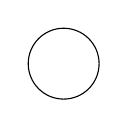
\begin{tikzpicture}
          \draw (0,0) circle [radius=0.45cm];
        \end{tikzpicture}

        \(S^1\)
      \end{minipage}
      \begin{minipage}{1.5in}
        \centering
        \includegraphics[scale=0.25]{sphere}

        \(S^n\) for \(n\ge2\)
      \end{minipage}

      \begin{minipage}{1.5in}
        \centering
        \includegraphics[scale=0.3]{torus}

        \(T=S^1\times S^1\)
      \end{minipage}
      \begin{minipage}{1.5in}
        \centering
        \includegraphics[scale=0.25]{dtorus}

        \(T\#T\)
      \end{minipage}
    \end{center}

  \item All are compact, but none are homeomorphic.
  \end{itemize}
\end{frame}

\begin{frame}
  \frametitle{Homotopy}
  \begin{itemize}
  \item Let \(I=[0,1]\subset\R\) imbued with the subspace topology.
  \item A continuous function \(F:X\times I\to Y\) between continuous functions \(f_1,f_2:X\to Y\).
  \item \(F(x,0)=f_1(x)\) and \(F(x,1)=f_2(x)\).
  \item \(f_1\) and \(f_2\) are homotopic \((f_1\simeq f_2)\).
  \item If \(f_2\) is a constant function then \(f_1\) is called nulhomotopic.
  \item A continuous deformation of \(f_1\) into \(f_2\) via a parameterized family of continuous functions.
  \end{itemize}
\end{frame}

\begin{frame}
  \frametitle{Homotopy Examples}
  \centering
  \begin{minipage}{2in}
    \centering
    \begin{tikzpicture}[scale=0.4]
      \begin{axis}[
          xmin=0,
          xmax=1,
          ymin=0,
          ymax=1,
          axis lines*=middle,
          xtick={0,1},
          ytick={0,1},
          ytick={0,1/5,2/5,3/5,4/5,1},
          yticklabels={\(0\),\(\frac{1}{5}\),\(\frac{2}{5}\),\(\frac{3}{5}\),\(\frac{4}{5}\),\(1\)},
          xlabel={\(I\)},
          ylabel={\(I\)},
          ylabel style={rotate=-90},
          clip=false
        ]
        \addplot [domain=0:1,red] {0} node [right] {\(f_1(x)=0\)};
        \addplot [domain=0:1,green] {1} node [right] {\(f_2(x)=1\)};
        \addplot [domain=0:1,dashed] {0.2};
        \addplot [domain=0:1,dashed] {0.4};
        \addplot [domain=0:1,dashed] {0.6};
        \addplot [domain=0:1,dashed] {0.8};
      \end{axis}
    \end{tikzpicture}

    \(F(x,t)=\pi_I(x,t)=t\)
  \end{minipage}
  \begin{minipage}{2in}
    \centering
    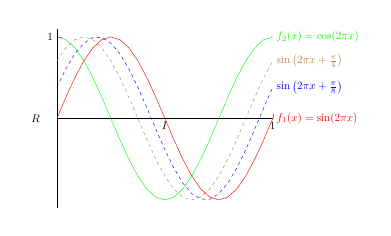
\begin{tikzpicture}[scale=0.4]
      \begin{axis}[
          xmin=0,
          xmax=1,
          ymin=-1.1,
          ymax=1.1,
          axis lines*=middle,
          xtick={0,1},
          ytick={0,1},
          xlabel={\(I\)},
          ylabel={\(R\)},
          xlabel style={above=0cm},
          ylabel style={rotate=-90},
          clip=false
        ]
        \addplot [domain=0:1,red] {sin(deg(2*pi*x))} node [right] {\(f_1(x)=\sin(2\pi x)\)};
        \addplot [domain=0:1,green] {cos(deg(2*pi*x))} node [right] {\(f_2(x)=\cos(2\pi x)\)};
        \addplot [domain=0:1,blue,dashed] {sin(deg(2*pi*x+pi/8))}
        node [right] {\(\sin\left(2\pi x+\frac{\pi}{8}\right)\)};
        \addplot [domain=0:1,brown,dashed] {sin(deg(2*pi*x+pi/4))}
        node [right] {\(\sin\left(2\pi x+\frac{\pi}{4}\right)\)};
      \end{axis}
    \end{tikzpicture}

    \(F(x,t)=\sin\left(2\pi x+t\frac{\pi}{2}\right)\)
  \end{minipage}

  \bigskip
  
  \begin{minipage}{2in}
    \centering
    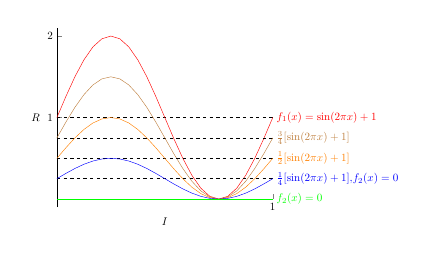
\begin{tikzpicture}[scale=0.4]
      \begin{axis}[
          xmin=0,
          xmax=1,
          ymin=-0.1,
          ymax=2.1,
          axis lines*=middle,
          xtick={0,1,2},
          ytick={0,1,2},
          xlabel={\(I\)},
          ylabel={\(R\)},
          ylabel style={rotate=-90},
          clip=false
        ]
        \draw [dashed] (0,1) -- (1,1);
        \addplot [domain=0:1,red] {sin(deg(2*pi*x))+1} node [right] {\(f_1(x)=\sin(2\pi x)+1\)};
        \draw [dashed] (0,3/4) -- (1,3/4);
        \addplot [domain=0:1,brown] {(3/4)*(sin(deg(2*pi*x))+1)} node [right] {\(\frac{3}{4}[\sin(2\pi x)+1]\)};
        \draw [dashed] (0,1/2) -- (1,1/2);
        \addplot [domain=0:1,orange] {(1/2)*(sin(deg(2*pi*x))+1)} node [right] {\(\frac{1}{2}[\sin(2\pi x)+1]\)};
        \draw [dashed] (0,1/4) -- (1,1/4);
        \addplot [domain=0:1,blue] {(1/4)*(sin(deg(2*pi*x))+1)} node [right]
                 {\(\frac{1}{4}[\sin(2\pi x)+1]\),\(f_2(x)=0\)};
        \addplot [domain=0:1,green] {0} node [right] {\(f_2(x)=0\)};
      \end{axis}
    \end{tikzpicture}

    \(F(x,t)=(1-t)[\sin(2\pi x)+1]\).
  \end{minipage}
\end{frame}

\begin{frame}
  \frametitle{Homotopy Properties}
  \begin{itemize}
  \item Homotopic is an equivalence relation.
  \item Let \([f]\) denote the equivalence class of continuous functions that are homotopic to \(f\).
  \item If \(Y\subset\R^n\) is convex then any two continuous \(f_1,f_2:X\to Y\) are homotopic via the straight-line
    homotopy:
    \[F(x,t)=(1-t)f_1(x)+tf_2(x)\]
    \begin{center}
      \includegraphics[scale=0.4]{slhomotopy}
    \end{center}
  \end{itemize}
\end{frame}

\begin{frame}
  \frametitle{Path Homotopy}
  \begin{itemize}
  \item \(f_1\) and \(f_2\) are paths in \(X\) with the same initial \((x_0)\) and final \((x_1)\) points.
  \item \(F:I\times I\to X\)
  \item \(F(x,0)=f_1(x)\) and \(F(x,1)=f_2(x)\)
  \item \(F(0,t)=x_0\) and \(F(1,t)=x_1\)

    \bigskip

    \begin{center}
      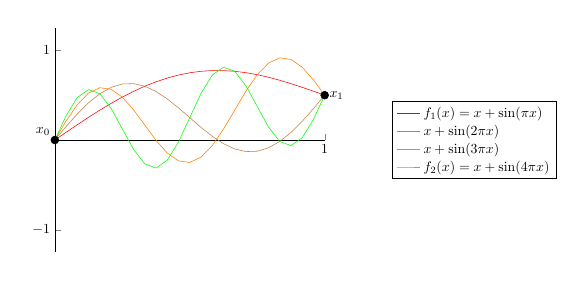
\begin{tikzpicture}[scale=0.5]
        \begin{axis}[
            xmin=0,
            xmax=1,
            ymin=-2.5,
            ymax=2.5,
            axis lines*=middle,
            xtick={0,1},
            ytick={-2,0,2},
            yticklabels={\(-1\),\(0\),\(1\)},
            legend style={at={(1.25,0.5)},anchor=west},
            legend cell align=left,
            clip=false
          ]
          \addplot [domain=0:1,red] {x+sin(deg(pi*x))};
          \addplot [domain=0:1,brown] {x+sin(deg(2*pi*x))};
          \addplot [domain=0:1,orange] {x+sin(deg(3*pi*x))};
          \addplot [domain=0:1,green] {x+sin(deg(4*pi*x))};
          \node [draw,circle,fill,inner sep=0,minimum size=0.2cm] at (0,0) {};
          \node [above left] at (0,0) {\(x_0\)};
          \node [draw,circle,fill,inner sep=0,minimum size=0.2cm] at (1,1) {};
          \node [right] at (1,1) {\(x_1\)};
          \legend{\(f_1(x)=x+\sin(\pi x)\),\(x+\sin(2\pi x)\),\(x+\sin(3\pi x)\),\(f_2(x)=x+\sin(4\pi x)\)}
        \end{axis}
      \end{tikzpicture}

      \bigskip

      \(F(s,t)=s+\sin[(3t+1)\pi s]\)
    \end{center}
  \end{itemize}
\end{frame}

\begin{frame}
  \frametitle{Product}
  \begin{itemize}
  \item \(f_1\) is a path from \(x_0\) to \(x_1\).
  \item \(f_2\) is a path from \(x_1\) to \(x_2\).
  \item Concatenates the two paths:
    \[f_1*f_2=\begin{cases}
    f_1(2t), & t\in\left[0,\frac{1}{2}\right] \\
    f_2(2t-1), & t\in\left[\frac{1}{2},1\right] \\
    \end{cases}\]
  \item Continuous by the pasting lemma.

    \bigskip

    \begin{center}
      \begin{tikzpicture}[dot/.style={draw,circle,fill,inner sep=0,minimum size=0.1cm}]
        \node [dot] (X0) at (0,0) {};
        \node [dot] (X1) at (2,1) {};
        \node [dot] (X2) at (4,2) {};
        \draw [blue] (X0) to [bend left] node [above] {\(f_1\)} (X1);
        \draw [green] (X1) to [bend right] node [below] {\(f_2\)} (X2);
        \node [below=1ex of X0] {\(x_0\)};
        \node [below=1ex of X1] {\(x_1\)};
        \node [above=1ex of X2] {\(x_2\)};
      \end{tikzpicture}
    \end{center}
  \end{itemize}
\end{frame}

\begin{frame}
  \frametitle{Product Groupoid}
  \begin{itemize}
  \item \(e_{x_0}(t)=x_0\)
  \item \(\bar{f}(t)=f(1-t)\)\qquad(reverse path)
  \item \(*\) is a partial function on \(X\): only works when \(f_1(1)=f_2(0)\).
  \item Forms a groupoid.
  \item Associative: \(([f]*[g])*[h]\) is defined if and only if \([f]*([g]*[h])\) is defined and if defined then
    they are equal.
  \item Identity: \([e_{x_0}]*[f]=[f]\) and \([f]*[e_{x_1}]=[f]\).
  \item Inverse: \([f]*[\bar{f}]=[e_{x_0}]\) and \([\bar{f}]*[f]=[e_{x_1}]\).
  \end{itemize}
\end{frame}

\begin{frame}
  \frametitle{Fundamental Group}
  \begin{itemize}
  \item A path that starts and ends at \(x_0\) is called a loop based at \(x_0\).
  \item For a topological space \(X\), select some \(x_0\in X\).
  \item Select all loops based at \(x_0\).
  \item The homotopic equivalence classes and \(*\) form a group: \(\pi_1(X,x_0)\) with identity \([e_{x_0}]\).
  \item For all \(x_0,x_1\in X\), \(\pi_1(X,x_0)\) is isomorphic to \(\pi_1(X,x_1)\).
  \item Topologically invariant (up to isomorphism).
  \item Only addresses the path component containing \(x_0\).
  \item If \(\pi_1(X,x_0)\) is not isomorphic to \(\pi_1(Y,y_0)\) then \(X\) and \(Y\) are not homeomorphic.
  \end{itemize}
\end{frame}

\begin{frame}
  \frametitle{Simply Connected}
  \begin{itemize}
  \item For all \(x_0\in X\), \(\pi_1(X,x_0)=\{[e_{x_0}]\}\) (trivial).
  \item Denoted by \(\pi_1(X,x_0)=0\).
  \item Any two paths with the same initial and final points are homotopic.
  \item Any convex subspace of \(\R^n\) is simply connected.
  \item In particular, all open balls in \(\R^n\) are simply connected: \(\pi_1(B(p,r),x_0)=0\).
  \end{itemize}
\end{frame}

\begin{frame}
  \frametitle{Non-homeomorphic Spaces}
  \begin{itemize}
  \item \(\pi_1(S^1,x_0)\sim\Z\)\qquad(times around the circle)

    \begin{center}
      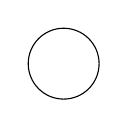
\begin{tikzpicture}
        \draw (0,0) circle [radius=0.45cm];
      \end{tikzpicture}
    \end{center}

  \item \(\pi_1(S^n,x_0)=0\) for \(n\ge2\)

    \begin{center}
      \includegraphics[scale=0.25]{sphere}
    \end{center}

  \item \(\pi_1(T=S^1\times S^1,x_0)\sim\Z\times\Z\)\qquad(abelian)

    \begin{center}
      \includegraphics[scale=0.25]{torus}
    \end{center}

  \item \(\pi_1(T\#T)\) is not abelian

    \begin{center}
      \includegraphics[scale=0.25]{dtorus}
    \end{center}
  \end{itemize}
\end{frame}

\end{document}
